% ==================///==================///==================///
% ==================/// LATEX'S STUFF
% ==================///==================///==================///

\documentclass[hungarian]{beamer}
\usepackage[T1]{fontenc}
\usepackage{babel}
\usepackage{graphicx}
\usepackage{hyperref}
\usepackage{stuki}

\usepackage{soul}

\usepackage{tikz}
\usetikzlibrary{shapes.multipart, positioning, arrows.meta}
\tikzset{list/.style={rectangle multipart, draw, minimum height=1cm, minimum width=1.5cm}}

\usepackage{amsfonts,amsmath,oldgerm}
\usetheme{_statale}
\usefonttheme[onlymath]{serif}

\newcommand{\testcolor}[1]{\colorbox{#1}{\textcolor{#1}{test}}~\texttt{#1}}
\newcommand{\hrefcol}[2]{\textcolor{cyan}{\href{#1}{#2}}}
\titlebackground*{assets/background}

\newcommand{\Ord}{\mathcal{O}}


% ==================///==================///==================///
% ==================/// SPLASH PAGE
% ==================///==================///==================///

\title{Algoritmusok I.}
\newcommand{\longauthor}{5. gyakorlat}
\author{Sipos Ágoston}
\newcommand{\correspondingauthor}{John Doe}
\newcommand{\email}{siposagoston@inf.elte.hu}
\renewcommand{\insertdate}{2026. október 7.}

% ==================///==================///==================///
% ==================/// START PRESENTATION
% ==================///==================///==================///

\begin{document}
\maketitle

\section{Beszúró rendezés}

\begin{frame}{Szemléltetés}

\begin{figure}
    \centering
    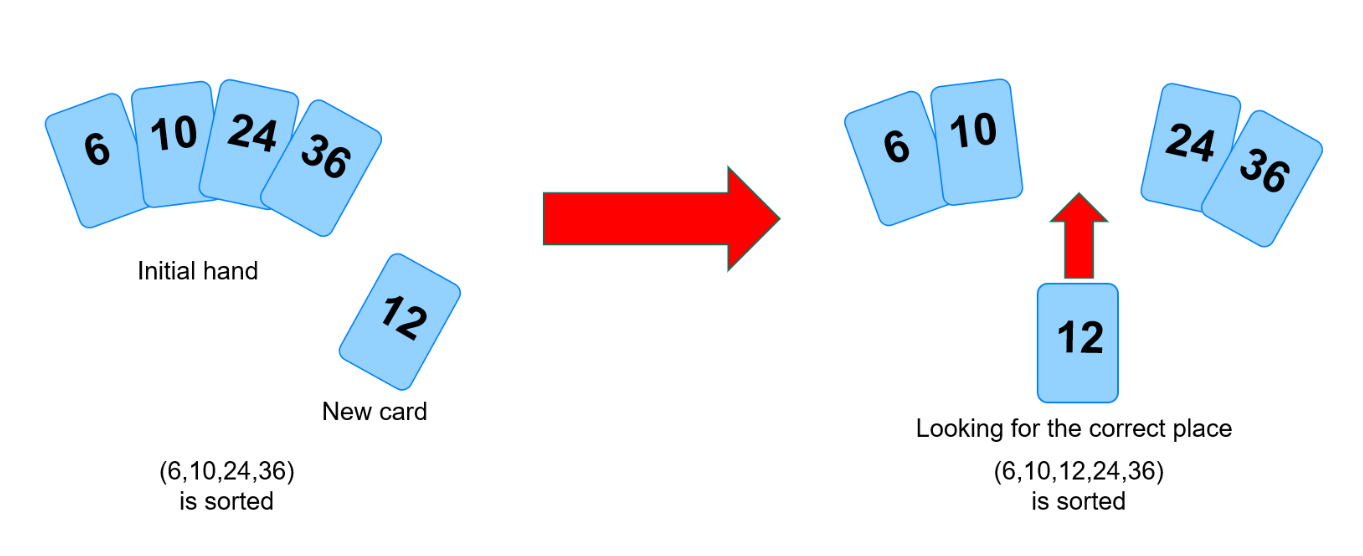
\includegraphics[width=1\linewidth]{assets/insertion.png}
\end{figure}

\end{frame}

\begin{frame}{Beszúró rendezés elve}

\begin{itemize}
    \item Tegyük fel, hogy az első (i-1) elem már rendezett
    \item Vegyük az i. elemet és szúrjuk be közéjük a megfelelő helyre
    \item Ha elértük a tömb\footnote{vagy lista is lehetne, de most foglalkozzunk a tömbökkel} végét, akkor az egész rendezett
\end{itemize}
    
\end{frame}

\begin{frame}{Naiv algoritmus}

A buborékrendezés analógiájára:

(0-tól indexelt tömb!)

\vspace{4mm}

\setlength{\stukiwidth}{5cm}
\begin{stukibox*}{naiveInsertionSort(A : $\mathcal{T}[n]$)}
\begin{WHILE}{4}{\stm{i = 1 \textrm{ to } n-1}}
\stm{j = i}
\begin{WHILE}{2}{\stm{j>0 \textrm{ and } A[j-1] > A[j]}}
\stm{swap(A[j-1], A[j])}
\stm{j = j-1}
\end{WHILE}
\end{WHILE}
\end{stukibox*}

\vspace{4mm}

Probléma: túl sok csere
    
\end{frame}

\begin{frame}{Algoritmus}

\begin{columns}
\begin{column}{0.5\linewidth}

\setlength{\stukiwidth}{6cm}
\begin{stukibox*}{insertionSort(A : $\mathcal{T}[n]$)}
\begin{WHILE}{8}{\stm{i = 1 \textrm{ to } n-1}}
\begin{IF}[70]{7}{\stm{A[i-1] > A[i]}}
\stm{x = A[i]}
\stm{A[i] = A[i-1]}
\stm{j = i-2}
\begin{WHILE}{2}{\stm{j\geq 0 \textrm{ and } A[j] > x}}
\stm{A[j+1] = A[j]}
\stm{j = j-1}
\end{WHILE}
\stm{A[j+1] = x}
\ELSE
\stm*{SKIP}
\end{IF}
\end{WHILE}
\end{stukibox*}

\end{column}
\begin{column}{0.5\linewidth}
Ötlet: a beszúrandó elemet vegyük ki egy segédváltozóba, a többi elemet toljuk eggyel jobbra, majd szúrjuk be a megfelelő helyre.

\vspace{1em}

Ezzel $k$ darab csere ($3k$ másolás) helyett csak $k+2$ másolást kell végeznünk. ($k$ az a szám, hogy mennyivel kell balra mozgatni a beszúrt elemet)

\end{column}
\end{columns}

\end{frame}

\begin{frame}{Jellemzés}

\begin{itemize}
    \item Minimális műveletigény: $mT(n) = \Theta(n)$ (ha minden elem a helyén van)
    \item Maximális, átlagos műveletigény: $aT(n) = MT(n) = \Theta(n^2)$ (a dupla ciklus miatt)
    \item Tárigény: $\Theta(1)$ (fix számú segédváltozó)
    \item Stabil rendezés
\end{itemize}
    
\end{frame}

\begin{frame}[t]{Lejátszás}

Rendezzük a következő tömböt beszúró rendezéssel!
$\langle 6, 5, 3, 1, 8, 7, 2, 4 \rangle$
    
\end{frame}

\section{Összefésülő rendezés}

\begin{frame}{Összefésülő rendezés}

\begin{columns}

\begin{column}{0.8\linewidth}

Neumann, 1945, EDVAC (állítólag az első, modern számítógépre megírt algoritmus)

\vspace{5mm}

,,Oszd meg és uralkodj'' típusú algoritmus: a problémát kisebb részproblémákra bontja, amíg el nem éri az alapesetet ami már triviálisan megoldható további rekurzió nélkül.

Összefésülés: a részproblémák megoldásait felhasználva kapjuk meg az alapprobléma megoldását.
\end{column}
\begin{column}{0.18\linewidth}

\begin{figure}
    \centering
    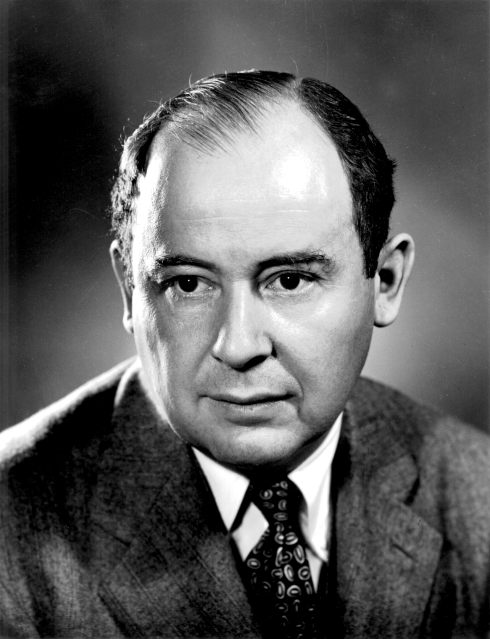
\includegraphics[width=1\linewidth]{assets/neumann.png}
\end{figure}

\end{column}

\end{columns}

\end{frame}

\begin{frame}{Ötlet}

Tegyük fel, hogy van két rendezett tömbünk, hogyan tudunk ezekből egy, mindkettő összes elemét tartalmazó tömböt kapni?

Tömbök összefésülése: elindulunk mindkét tömbön 1-1 indexszel, és amelyikben kisebb értéket látunk, azt átmásoljuk egy új tömbbe, és léptetjük azt az indexet.

\end{frame}

\begin{frame}{Vizualizáció}

\centering
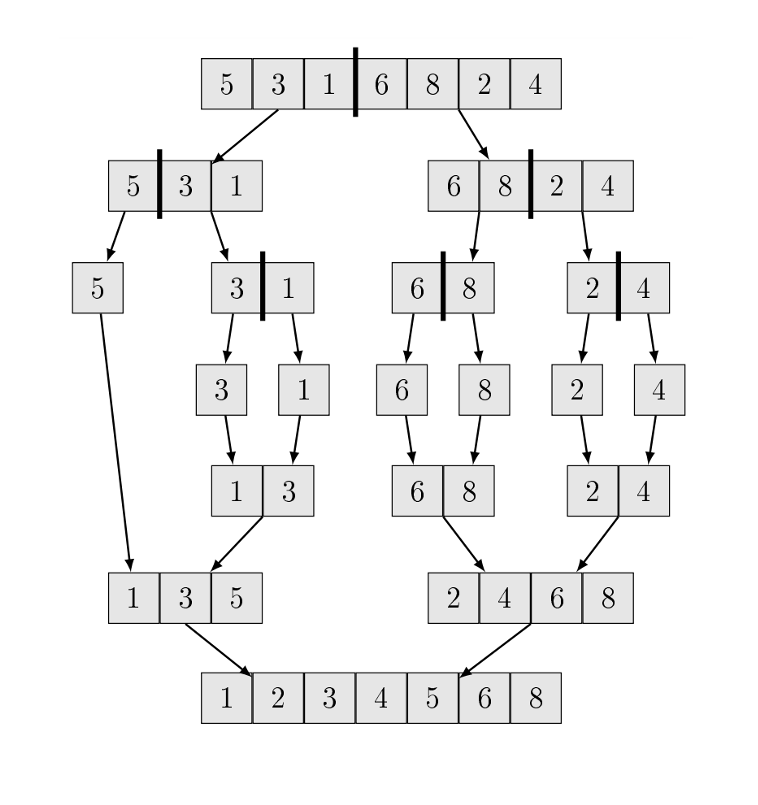
\includegraphics[height=0.8\paperheight]{assets/mergesort.png}
    
\end{frame}

\begin{frame}{Folyamat}

Rendezetlen tömb:

\begin{tabular}{|c|c|c|c|c|c|}
    \hline
    31 & 25 & 59 & 11 & 93 & 58 \\
    \hline
\end{tabular}

\vspace{5mm}

Kettéválasztjuk:

\begin{tabular}{|c|c|c||c|c|c|}
    \hline
    31 & 25 & 59 & 11 & 93 & 58 \\
    \hline
\end{tabular}

\vspace{5mm}

A két résztömböt az algoritmus, rekurzívan meghívva önmagát, rendezi (ezt még lehetne tovább részletezni):

\begin{tabular}{|c|c|c||c|c|c|}
    \hline
    25 & 31 & 59 & 11 & 58 & 93 \\
    \hline
\end{tabular}

\vspace{5mm}

A két rendezett résztömböt összefuttatjuk:

\begin{tabular}{|c|c|c|c|c|c|}
    \hline
    11 & 25 & 31 & 58 & 59 & 93 \\
    \hline
\end{tabular}

\end{frame}

\begin{frame}{Összefuttatás}

\begin{columns}

\begin{column}{0.3\linewidth}

Az A tömb [a1;b1] és [a2;b2] részsorozatának összefuttatása a B tömb [a1;b2] részsorozatába (tegyük fel hogy $a2 = b1 + 1$)

\end{column}

\begin{column}{0.6\linewidth}

\begin{stukibox*}{merge(A, a1, b1, a2, b2)}
\stm{i1 = a1; i2 = a2; i = a1}
\begin{WHILE}{3}{\stm{i1 \leq b1 \mathrm{~and~} i2 \leq b2}}
    \begin{IF}{2}{\stm{A[i1] < A[i2]}}
        \stm{B[i] = A[i1]}
        \stm{i = i+1;~i1 = i1+1}
    \ELSE
        \stm{B[i] = A[i2]}
        \stm{i = i+1;~i2 = i2+1}
    \end{IF}
\end{WHILE}
\begin{IF}{3}{\stm{i1 \leq b1}}
    \begin{WHILE}{2}{\stm{i1 < b1}}
        \stm{B[i] = A[i1]}
        \stm{i = i + 1; i1 = i1 + 1}
    \end{WHILE}
\ELSE
    \begin{WHILE}{2}{\stm{i2 < b2}}
        \stm{B[i] = A[i2]}
        \stm{i = i + 1; i2 = i2 + 1}
    \end{WHILE}
\end{IF}
\end{stukibox*}

\end{column}

\end{columns}
    
\end{frame}

\begin{frame}{Elemzés}

Összefuttatás algoritmusa: $\Ord(n)$

Rekurzió mélysége: $\log_2 n$

Minden szintjén a rekurziónak néhány, együttvéve $n$ hosszú összefuttatást végzünk, ez még mindig lineáris.

Összegezve: műveletigény $\Ord(n \cdot \log n)$

Segédtömb szükséges az összefuttatások elvégzéséhez: tárigény $\Ord(n)$

\end{frame}

\begin{frame}[t]{Lejátszás}

Rendezzük a következő tömböt összefésülő rendezéssel!
$\langle 6, 5, 3, 1, 8, 7, 2, 4 \rangle$
    
\end{frame}

\section{Gyorsrendezés}

\begin{frame}{Ötlet}


\begin{columns}

\begin{column}{0.8\linewidth}

Hoare, 1961

\vspace{5mm}

Szintén ,,oszd meg és uralkodj'' elven működik.

Minden lépésben kiválaszt egy pivot elemet, amit úgy helyez el, hogy a nála kisebbek előtte, a nála nagyobbak utána legyenek.

Ezután rekurzívan meghívja önmagát a két még nem rendezett részsorozatra.


\end{column}
\begin{column}{0.18\linewidth}

\begin{figure}
    \centering
    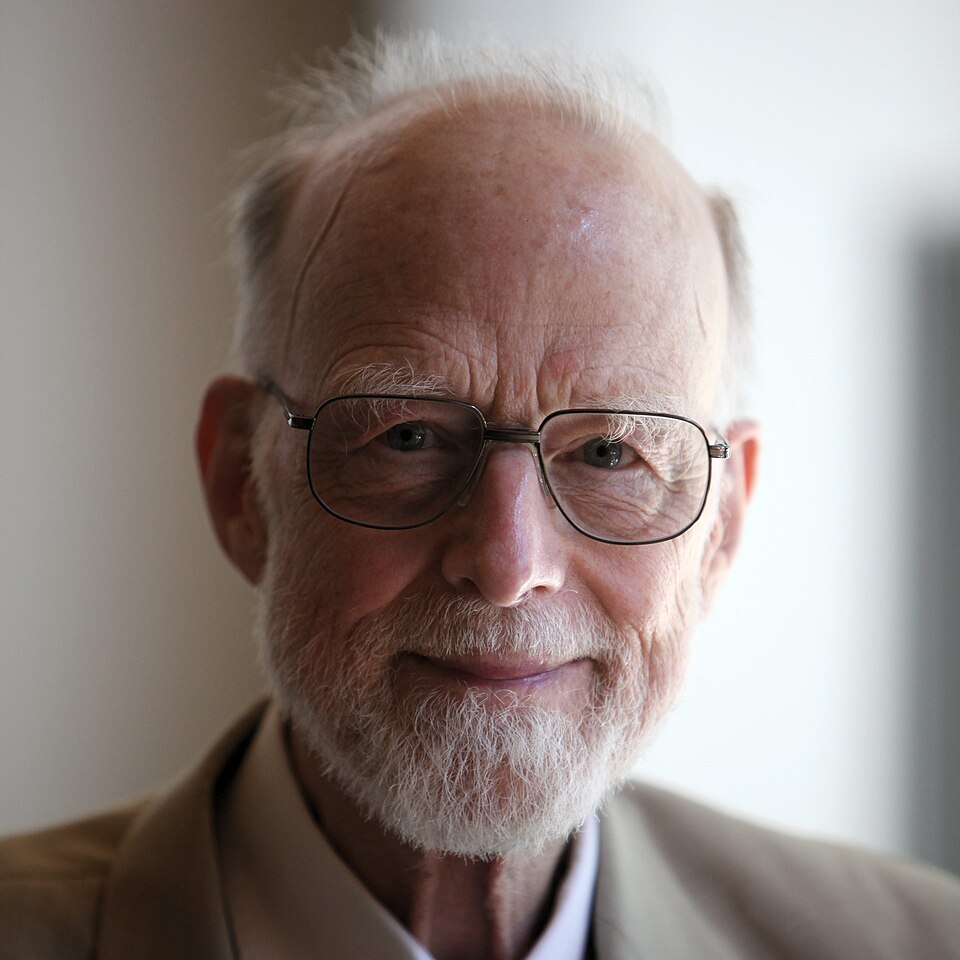
\includegraphics[width=1\linewidth]{assets/hoare.png}
\end{figure}

\end{column}

\end{columns}

\end{frame}


\begin{frame}{Folyamat}

Rendezetlen tömb:

\begin{tabular}{|c|c|c|c|c|c|}
    \hline
    31 & 25 & 59 & 11 & 93 & 58 \\
    \hline
\end{tabular}

\vspace{5mm}

Pivot elem választása:

\begin{tabular}{|c||c|c|c|c|c|}
    \hline
    31 & 25 & 59 & 11 & 93 & 58 \\
    \hline
\end{tabular}

\vspace{5mm}

A pivot elem elé, és mögé válogatjuk a többi elemet:

\begin{tabular}{|c|c||c||c|c|c|}
    \hline
    25 & 11 & 31 & 59 & 58 & 93 \\
    \hline
\end{tabular}

\vspace{5mm}

A két résztömböt az algoritmus, rekurzívan meghívva önmagát, rendezi (ezt még lehetne tovább részletezni):

\begin{tabular}{|c|c||c||c|c|c|}
    \hline
    11 & 25 & 31 & 58 & 59 & 93 \\
    \hline
\end{tabular}

\end{frame}

\begin{frame}{Elemek válogatása}

\begin{columns}

\begin{column}{0.3\linewidth}

Az elemek szétválogatása az A tömb [a; b] részsorozatában, helyben, úgy hogy az A[i] pivot elem előtt a nála kisebb, utána a nagyobb elemek szerepeljenek.

A végén i-ben a pivotelem új helye lesz.

\end{column}

\begin{column}{0.6\linewidth}

\vspace{-12mm}

\begin{stukibox*}{partition(A, a, b, i)}
\stm{\textrm{swap}(A[i], A[b])}
\stm{i = a}
\begin{WHILE}{1}{\stm{i < b \textrm{~and~} A[i] \leq A[b]}}
    \stm{i = i + 1}
\end{WHILE}
\begin{IF}[80]{7}{\stm{i < b}}
    \stm{j = i + 1}
    \begin{WHILE}{4}{\stm{j < b}}
        \begin{IF}{2}{\stm{A[j] < A[b]}}
            \stm{\textrm{swap}(A[i], A[j])}
            \stm{i = i + 1}
        \ELSE
            \stm*{SKIP}
        \end{IF}
        \stm{j = j + 1}
    \end{WHILE}
    \stm{\textrm{swap}(A[i], A[b])}
\ELSE
    \stm*{SKIP}
\end{IF}
\end{stukibox*}

\end{column}

\end{columns}

\end{frame}

\begin{frame}{Elemzés}

Szétválogatás műveletigénye: $\Ord(n)$

Rekurzió mélysége: legrosszabb esetben (mindig a legnagyobb / legkisebb elem a pivot) $\Ord(n)$; várhatóan $\Ord(\log n)$

Tehát $mT(n) = aT(n) = \Ord(n \log n)$, $MT(n) = \Ord(n^2)$

Tárigény: $\Ord(1)$, nem kell segédtömb

Ebben a formában nem stabil (a szétválogatás során össze-vissza dobáljuk az elemeket)
    
\end{frame}

\begin{frame}[t]{Lejátszás}

Rendezzük a következő tömböt gyorsrendezéssel!
$\langle 8, 12, 5, 14, 10, 2, 9, 17, 3, 9 \rangle$


\end{frame}

\end{document}
